\documentclass{standalone}
\usepackage{xcolor}
\usepackage{verbatim}
\usepackage[T1]{fontenc}
\usepackage{graphics}
\usepackage{hyperref}
\newcommand{\code}[1]{\texttt{#1}}
\newcommand{\R}{R}
\newcommand{\pkg}[1]{#1}
\newcommand{\CRANpkg}[1]{\pkg{#1}}%
\newcommand{\BIOpkg}[1]{\pkg{#1}}
\usepackage{amsmath,amssymb,array}
\usepackage{booktabs}
\usepackage{tikz}
\usetikzlibrary{decorations.pathreplacing}


\begin{document}
\nopagecolor
   \tikzset{
	dot diameter/.store in=\dot@diameter,
	dot diameter=2pt,
	dot spacing/.store in=\dot@spacing,
	dot spacing=4.5pt,
	dots/.style={
		line width=\dot@diameter,
		line cap=round,
		dash pattern=on 0pt off \dot@spacing
	}
}
	\centering

	%\begin{changemargin}{1cm}{1cm}
	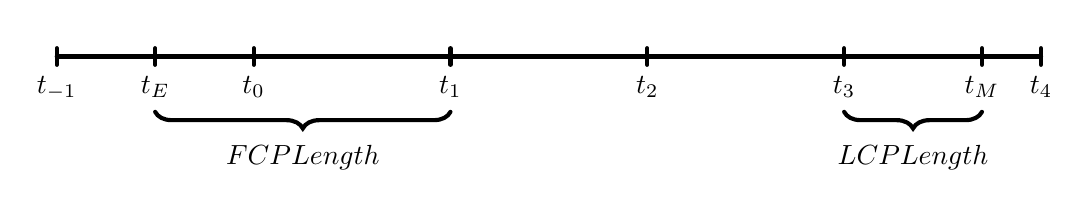
\begin{tikzpicture}[line width=1.5pt, line cap=round] 
	%	\tikzstyle{every node}=[font=\small]
	% draw horizontal lines
	\draw (0,0) -- (12.5,0);
	% draw vertical lines
	\foreach \x in {0,1.25,2.5,5,7.5,10,11.75,12.5}
	\draw (\x cm,3pt) -- (\x cm,-3pt);
	% draw nodes
	\draw (0,0) node[below=3pt] {$ t_{-1} $} node[above=3pt] {$  $};
	\draw (1.25,0) node[below=3pt] {$ t_{E} $} node[above=3pt] {$  $};
	\draw (2.5,0) node[below=3pt] {$ t_{0} $} node[above=3pt] {$  $};
	\draw (5,0) node[below=3pt] {$ t_{1} $} node[above=3pt] {$  $};
	\draw (7.5,0) node[below=3pt] {$ t_{2} $} node[above=3pt] {$  $};
	\draw (10,0) node[below=3pt] {$ t_{3} $} node[above=3pt] {$  $};
	\draw (11.75,0) node[below=3pt] {$ t_{M} $} node[above=3pt] {$  $};
	\draw (12.5,0) node[below=3pt] {$ t_{4} $} node[above=3pt] {$  $};
	\draw[decorate, decoration={brace,mirror,amplitude=6pt}, yshift=-20pt]  (1.25,0) -- node[below=8pt] {$ FCPLength $}  (5,0);
	\draw[decorate, decoration={brace,mirror,amplitude=6pt}, yshift=-20pt]  (10,0) -- node[below=8pt] {$ LCPLength $}  (11.75,0);
	%\draw[thick,red,decorate,decoration={brace,amplitude=-12pt}] (3,2pt) -- (4.5,-12pt) node[midway, below,yshift=-12pt,]{Test};
	\end{tikzpicture}
\end{document}
